%!TEX root = ../dissertation.tex

\chapter{Evaluation}
\label{chapter:evaluation}
% Introduce evaluation...
% Main goals
% Setup used

After the implementation of this solution, explained in chapter \ref{chapter:implementation}, some experiments were performed in order to test it.
When the mobile app for end users,
described in section \ref{sec:solution_mobile_app_for_end_users}, scans for beacons, it tries to find to which Smart Places they belong to and notifify the user if at least one was found.
If the user touches one of those notifications, the interface to the selected Smart Place is shown and the user can start to interact with it.
Then, the app will keep on scanning for beacons but now, only the nearest one is relevant and the app request the data, associated to that beacon in the context of the given Smart Place.
This means that, somehow, it has into account the physical distance between the device and the beacons.
The library used to handle the beacons has a method to get the distance from a given beacon.
There is a need to check if the distance's value we get from this library is reliable.
The same app needs to run, in background, in order to let the user be notified when he/she is nearby any Smart Place, instead of requiring his/her interaction.
However, as any service running in background, it can have a negative impact on the mobile device's resources usage, such as, battery.
A set of experiments was performed to evaluate the overhead introduced by our solution and if it is acceptable, having an app, running in background, scanning for beacons.

In section \ref{sec:evaluation_setup}, we describe the setup used, such as the mobile device and the set of beacons.
Then, we present two sets of experiments.
The first one, presented in section \ref{sec:evaluation_nearest_beacon}, was performed in order to get a good insight about the reliability of the distance value we get from the beacons library \gls{API}, to see if Smart Places that rely on the nearest beacon, would work as expected.
The other set of experiments, introduced in section \ref{sec:evaluation_energy_consumption}, measured data transferred (sent and received) and power drain, to take conclusions about if the energy consumption overhead, introduced by our solution, would be acceptable in a daily basis usage and the relation between the data transferred, due to requests to the backend, and the battery consumption.
For each set of experiments, we present the methodology, such as the conditions and measures taken and the results.
Finnaly, section \ref{sec:evaluation_summary} summarizes this chapter.

\section{Setup}
\label{sec:evaluation_setup}
In the evaluation process, a smartphone and a set of three beacons were used.
The smartphone was a \tm{Motorola}
Moto G\footnote{http://www.gsmarena.com/motorola\_moto\_g-5831.php}.
This device has the following specifications:
\begin{description}
  \item[\gls{CPU}:] Quad-core 1.2 GHz Cortex-A7\footnote{http://www.arm.com/products/processors/cortex-a/cortex-a7.php}
  \item[\gls{GPU}:] Adreno 305
  \item[\gls{RAM}:] 1 \gls{GB}
  \item[Internal storage:]: 16 \gls{GB}
  \item[Screen:] 4.5 inches
  \item[Battery:] Non-removable Li-Ion 2070 \gls{mAh} battery
  \item[\gls{OS}:] Android 5.0.2 (Lollipop\footnote{https://www.android.com/versions/lollipop-5-0})
\end{description}

As already described, in chapter \ref{chapter:implementation}, we have used three beacons from \tm{Estimote}.

\section{Nearest Beacon Detection}
\label{sec:evaluation_nearest_beacon}
Our solution relies on a library, which its \gls{API} allows us to get the distance from a given beacon.
However, this value is related to the signal's strength, that comes from the beacon.
We performed a set of experiments to verify how reliable was this value and if we can use that value to compute which beacon is the nearest one.
Next, related to this set of experiments, we describe the methodology used and outline the results.

\subsection{Methodology}
\label{sub:evaluation_nearest_beacon_methodology}
The set of experiments, summarized in Table~\ref{tab:experiments_nearest_beacon}, try to test if the mobile app can detect the nearest beacon.
In these experiments, the Smart Musem example was used.
In each experiment, it ran for 5 minutes using 10 seconds as the interval between each scan.
10 seconds was chosen because it is a reasonable value to walk in the museum to have enough time to perform any computation, that was needed, after each scan.
In each scan, the app executes code that checks if the scanned beacons were already detected in a previous scan. If they were not, the data associated to those beacons is requested from the backend, which, depending on the internet connection, can take some time.
This time interval between each scan seemed reasonable to make the request and compute the result until a new scan occurs.
With a much lower value, we could have a situation where another scan occurs while the previous one was not computed yet.
Running the experiment for 5 minutes, with the mentioned interval between each scan, allowed us to have more than 20 scans.
Then, in Android Studio log output, it was possible to check how many times each beacon was detected as the nearest one.

The smartphone and the three beacons were disposed in a layout, where each beacon was equally distant from each other and the smartphone was close to one of them, as shown in Figure~\ref{fig:layout_experiments_nearest_beacon}, where value d, is the distance between beacons.
The names below each beacon (ice, blueberry and mint), were defined by \tm{Estimote} in
the developer pack.
In this first set of experiments, the value d starts at 50 centimeters and is increased by 50 centimeters in each experiment until the 4th one where it is 2 meters.

\begin{table}[]
\centering
\begin{tabular}{@{}|l|c|c|c|c|@{}}
\toprule
\multicolumn{1}{|c|}{}                & \multicolumn{4}{c|}{{\bf Experiments}}                                                                            \\ \midrule
\multicolumn{1}{|c|}{{\bf Variables}} & {\bf 1}                     & {\bf 2}                   & {\bf 3}                     & {\bf 4}                   \\ \midrule
Events                                & \multicolumn{4}{c|}{\begin{tabular}[c]{@{}c@{}}For each beacon, \\ how many times \\ it was scanned\end{tabular}} \\ \midrule
Number of beacons                     & \multicolumn{4}{c|}{3}                                                                                            \\ \midrule
Interval between each scan (seconds)  & \multicolumn{4}{c|}{10}                                                                                           \\ \midrule
Experiment duration (minutes)         & \multicolumn{4}{c|}{5}                                                                                            \\ \midrule
Distance between beacons (meters)     & \multicolumn{1}{r|}{0.5}    & \multicolumn{1}{r|}{1}    & \multicolumn{1}{r|}{1.5}    & \multicolumn{1}{r|}{2}    \\ \bottomrule
\end{tabular}
\caption[Nearest beacon experiments summary]{Experiments to get the accuracy of the method to get the nearest beacon}
\label{tab:experiments_nearest_beacon}
\end{table}


\begin{figure}[!ht]
  \centering
    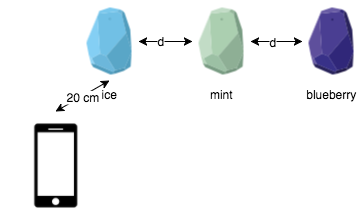
\includegraphics[width=0.5\textwidth, keepaspectratio]{images/nearest_beacon}
    \caption[Layout for experiments of nearest beacon]{Layout used for the experiments to get the accuracy of the distance value}
    \label{fig:layout_experiments_nearest_beacon}
\end{figure}

\subsection{Results}
\label{sub:evaluation_nearest_beacon_results}
The mobile app for end users scans for beacons but only requests data for the nearest one. To get the nearest one, it has to rely on the signal strength to calculate the distance. We performed 4 experiments in order to try to get the accuracy of the mechanism that calculates the distance that the mobile device is from a given beacon.
The results of these experiments are summarized in Table~\ref{tab:results_nearest_beacon}, where it is possible to see, for each beacon, how many times it was detected as the nearest one.

Taking into account the layout that was used (see Figure~\ref{fig:layout_experiments_nearest_beacon}), the nearest beacon was the one with name ``ice'' (the blue one).
From Table~\ref{tab:results_nearest_beacon}, it was possible to create the graphic shown in Figure~\ref{fig:results_experiments_nearest_beacon}, which shows that, as we increase the distance between beacons, the accuracy to detect the nearest beacon also increases.
In all experiments, this beacon was detected, as the nearest one, at least 50\% off all scans performed.
The only difference between all experiments is the distance between beacons.
We can conclude that, it is recommended that the beacons are, at least, 1.5m or 2m distant from each other.

% Please add the following required packages to your document preamble:
% \usepackage{booktabs}
\begin{table}[]
\centering
\begin{tabular}{@{}|c|r|r|r|r|r|@{}}
\toprule
{\bf } & \multicolumn{3}{c|}{{\bf Beacons}} & \multicolumn{2}{c|}{{\bf }} \\ \midrule
{\bf Experiments} & \multicolumn{1}{c|}{{\bf Ice}} & \multicolumn{1}{c|}{{\bf Mint}} & \multicolumn{1}{c|}{{\bf Blueberry}} & \multicolumn{1}{c|}{{\bf Total Scans}} & \multicolumn{1}{c|}{{\bf \% Correct}} \\ \midrule
{\bf 1} & 11 & 7 & 4 & 22 & 50.00\% \\ \midrule
{\bf 2} & 11 & 8 & 0 & 19 & 57.89\% \\ \midrule
{\bf 3} & 14 & 7 & 0 & 21 & 66.67\% \\ \midrule
{\bf 4} & 15 & 1 & 0 & 16 & 93.75\% \\ \bottomrule
\end{tabular}
\caption{Results of experiments about the accuracy to get the nearest beacon}
\label{tab:results_nearest_beacon}
\end{table}


\begin{figure}[!ht]
  \centering
    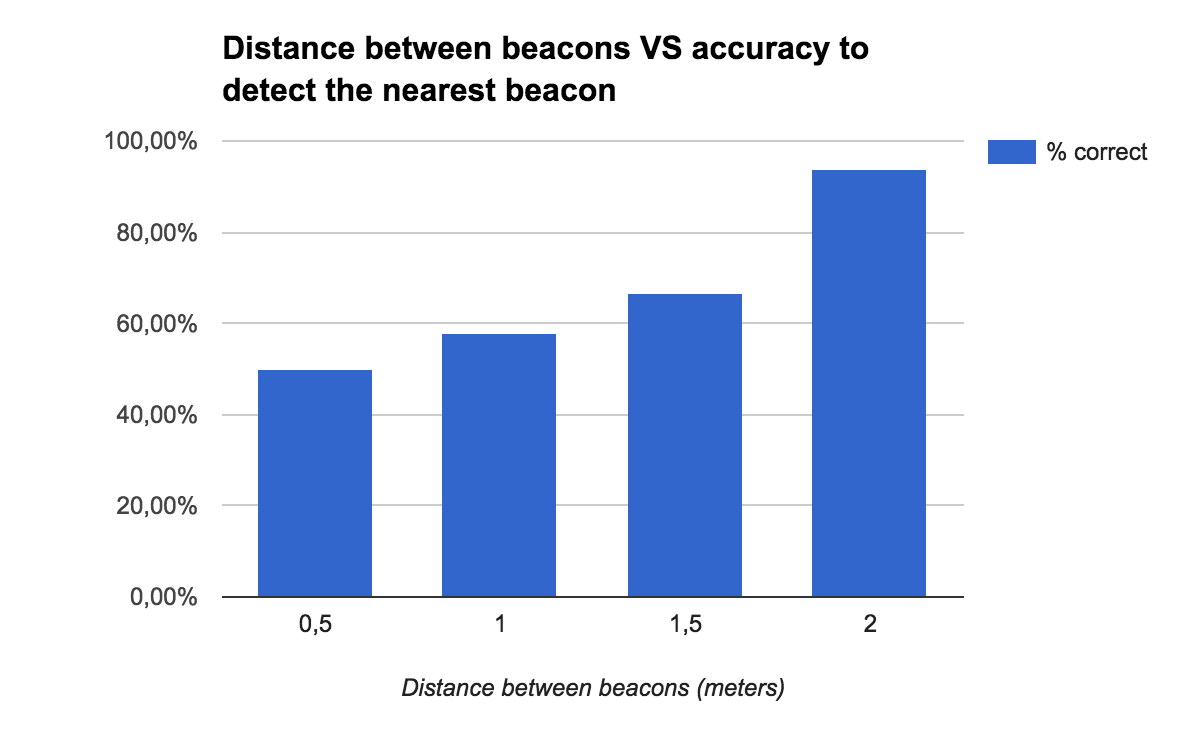
\includegraphics[width=0.5\textwidth, keepaspectratio]{images/results_nearest_beacon}
    \caption[Distance between beacons vs Accuracy]{Relation between distance between beacons and accuracy to detect the nearest beacon}
    \label{fig:results_experiments_nearest_beacon}
\end{figure}

In an environment, where the beacons are close to each other, our solution might not work as expected.
For instance, in the previously described Smart Restaurant example,
the tables should not be close to each other. This is not always possible because, some restaurants try to optimize space and have tables as much close to each other as possible.
In the Smart Museum example, two objects, in a given exhibition, should not be close to each other.
Otherwise, the visitor would be notified about an object and he might be looking at another one.
This error can be avoided using solutions such as Estimote Indoor \gls{SDK}\footnote{http://github.com/Estimote/iOS-Indoor-SDK} that can be used to obtain the physical indoors positon of the user.
However, it is only available for iOS.

\section{Energy Consumption}
\label{sec:evaluation_energy_consumption}
Another important aspect of this solution is the battery consumption.
Since our mobile app for end users runs on background to scan for nearby beacons, that can have a negative impact on the device's battery. If the user notice that the battery drains too fast, he/she will not use this solution.
Similar to section \ref{sec:evaluation_nearest_beacon}, in the next sub sections, we describe the metholodogy used and explain the results obtained in these experiments.

\subsection{Methodology}
\label{sub:evaluation_energy_consumption_methodology}
Table~\ref{tab:experiments_battery} outlines the experiments performed to evaluate the battery consumption.
Figure~\ref{fig:layout_experiments_battery_consumption} shows the layout used for this group of experiments.
We have used the same beacons, as in the experiments described in section \ref{sec:evaluation_nearest_beacon}.
The beacons are equally distant, 25 cm, from each other.
The smartphone is at the same distance from the beacon in the middle, the green one named mint.
We performed six experiments.
In each one the app was turned on and ran for 1 hour, in background mode, scanning for beacons in order to discover nearby Smart Places.
The first two used \gls{WiFi} data connection.
The remaining used \gls{3G} mobile network.
Different data connection means can lead to different energy consumptions.
We need to understand which connection, \gls{WiFi} or \gls{3G}, drains more power.
If it is \gls{3G}, the user might only use our solution if he/she is connected to a \gls{WiFi} \gls{AP}.
We want our mobile app to be always turned on scanning for nearby Smart Places.
Using it only when \gls{WiFi} is available would make its usage very limited and the user would not take the full advantage of it, because he/she needs be aware that a \gls{WiFi} \gls{AP} is available and turn the mobile app on again.
We tested two values for the interval between each scan, 5 minutes, because it is the default value that the beacons library use in background mode, and 2 and half minutes.
The second value is half the first in order to see how much more power is drained when we set a smaller value for the interval between each scan.
Trying to find a smaller interval is important because it will reduce the probability that the user was not able to discover a nearby Smart Place.

The following scenarios were tested:
\begin{itemize}
  \item
  When the user stays in the same Smart Place the entire experiment;
  % Explain better
  \item
  When the user moves from one Smart Place to another, at each two and half minutes.
  % Explain better
\end{itemize}

% Please add the following required packages to your document preamble:
% \usepackage{booktabs}
\begin{table}[]
\centering
\begin{tabular}{@{}|c|c|c|c|c|@{}}
\toprule
\multicolumn{1}{|l|}{}                     & \multicolumn{4}{c|}{{\bf Experiments}}                                                                \\ \midrule
{\bf Variables}                            & {\bf 1}                  & {\bf 2}                & {\bf 3}                  & {\bf 4}                \\ \midrule
{\bf Data connection type}                 & \multicolumn{2}{c|}{WiFi}                         & \multicolumn{2}{c|}{3G}                           \\ \midrule
{\bf Interval between each scan (minutes)} & \multicolumn{1}{r|}{2.5} & \multicolumn{1}{r|}{5} & \multicolumn{1}{r|}{2.5} & \multicolumn{1}{r|}{5} \\ \midrule
{\bf Experiment duration (hours)}          & \multicolumn{4}{c|}{1}                                                                                \\ \bottomrule
\end{tabular}
\caption[Battery consumption results]{Summary of experiments to get the battery consumption when the mobile
app is scanning for beacons in the background}
\label{tab:experiments_battery}
\end{table}


\begin{figure}[!ht]
  \centering
    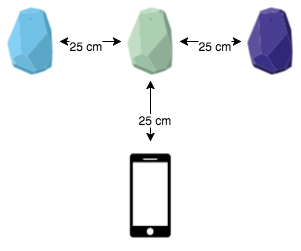
\includegraphics[width=0.5\textwidth, keepaspectratio]{images/experiments_battery_layout}
    \caption[Layout for experiments of battery consumption]{Layout used for the experiments to get the battery consumption}
    \label{fig:layout_experiments_battery_consumption}
\end{figure}

As already mentioned, for the evaluation process, we have used three \tm{Estimote} beacons.
The mobile app for end users has a cache that stores the beacons that were already scanned.
This way, repeated communications with the backend are avoided.
Data communications, \gls{WiFi} or \gls{3G}, are the major source of battery drain, as suggested in studies, such as \cite{energy}.
To test both scenarios, we would need more than three beacons spread along a big space.
Instead, we simulated the user walking, passing by multiple Smart Places, just by cleaning the cache, at each two and half minutes.
This forced the app to make requests to the backend each time the three beacons were detected, allowing us to understand the impact of these requests on the power drain.
We used Battery Historian\footnote{https://developer.android.com/tools/performance/batterystats-battery-historian/index.html} to to measure the power drain and how much data was transferred (sent and received). This tool allows developers to get the percentage of power drain of any application.

\subsection{Results}
\label{sub:evaluation_energy_consumption_results}
As already mentioned, in our solution, there is a mobile app that periodically, scans for beacons, in the background.
As any service running in background, it can imply some overhead in terms of energy.
Following the methodology, explained before, we evaluated the battery consumption.
For the first scenario, when the user stays in the same Smart Place, during each experiment, the results are summarized in Table~\ref{tab:results_battery_stopped}, where we can see, for each variation of data connection type (\gls{WiFi} and \gls{3G}) and interval between each scan, the values obtained for power drain and data transferred.
From this table, it was possible to create the graphic, shown in Figure~\ref{fig:results_battery_stopped}.
The battery consumption using \gls{WiFi} is almost zero.
However, when using \gls{3G}, the battery consumption raises more than 30 times than using \gls{WiFi}.

% Please add the following required packages to your document preamble:
% \usepackage{booktabs}
\begin{table}[]
\centering
\begin{tabular}{@{}lrrlrr@{}}
\toprule
\textbf{Variables}                                                                          & \multicolumn{5}{c}{\textbf{Results}}                  \\ \midrule
\textbf{Data connection type}                                                               & \multicolumn{2}{c}{WiFi} &   & \multicolumn{2}{c}{3G} \\ \cmidrule{2-3} \cmidrule{5-6}
\textbf{Interval between each scan}                                                         & 2m30s       & 5m         &   & 2m30s      & 5m        \\
\textbf{Computed power drain (\%)}                                                          & 0.00        & 0.00       &   & 0.40       & 0.29      \\
\textbf{\begin{tabular}[c]{@{}l@{}}Data transferred \\ (KB sent and received)\end{tabular}} & 34.96       & 31.10      &   & 21.67      & 35.28     \\ \bottomrule
\end{tabular}
\caption[Power drain when the user is not moving]{Results of the experiments to get the battery consumption in the scenario where the user stays in the same Smart Place}
\label{tab:results_battery_stopped}
\end{table}


\begin{figure}[!ht]
  \centering
    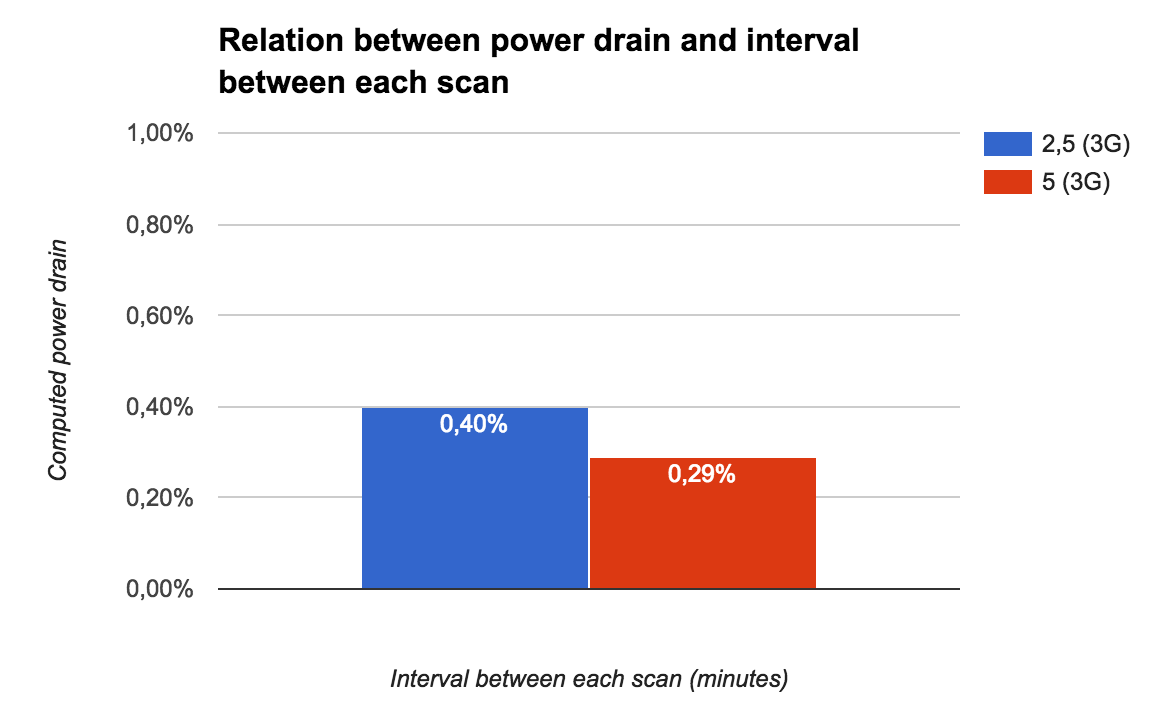
\includegraphics[width=0.8\textwidth, keepaspectratio]{images/results_battery_stopped}
    \caption[Power drain when the user does not move]{Relation between power drain and interval between each scan in the scenario where the user stays in the same Smart Place}
    \label{fig:results_battery_stopped}
\end{figure}

From this results, it is possible to conclude that, our solution, introduces the most overhead when using \gls{3G} as the mean to perform data communications, such as, communications with the backend.
For each data connection type (\gls{WiFi} and \gls{3G}), we tested two values for the interval between each scan for nearby beacons.
We can observe, when we decrease the interval between each scan in half, the battery consumption increases in 0.1\%.
Taking into account that we spent one hour, in each experiment, assuming that the values, for the power drain, grow lineary, it is possible to say that, for two and half and five minutes, in interval between each scan, we would have 6.96\% and 9.6\%, in 24 hours, of power drain, respectively.
The values are still low but these values can demotivate the usage of our solution because, it is very likely that the users already have mobile apps, that use mobile data, already installed in their devices.

Regarding the second scenario, where the user moves from one Smart Place to another, at each two and half minutes.
Table~\ref{tab:results_battery_walking}, shows the results for this scenario. Here, we got more power drain than in the previous scenario.
These results shows that, the more communication with the backend is required, more power our solution drains.
Once more, using \gls{WiFi}, we have got almost zero power drain.
However, simillary to the results in the previous scenario, there is more power drain using \gls{3G}.
Graphic shown in Figure~\ref{fig:results_battery_walking} shows that, using two minutes and half of interval between each scan, we got more 0.71\% than using five minutes.
As happened before, there is more power drain when we increase the interval between each scan.
Assuming a linear growth of power drain, in the worst case, after 24 hours, there is 65.04\% of power drain.
In this case, we got more than 60 times the power drain than the worst case in the previous scenario.
With this value, our solution can be considered unacceptable for a daily basis usage, that is, having the mobile app always running in background.

% Please add the following required packages to your document preamble:
% \usepackage{booktabs}
\begin{table}[]
\centering
\begin{tabular}{@{}|l|r|r|r|r|@{}}
\toprule
{\bf }                                        & \multicolumn{4}{c|}{{\bf Results}}                  \\ \midrule
{\bf Data connection type}                    & \multicolumn{2}{c|}{WiFi} & \multicolumn{2}{c|}{3G} \\ \midrule
{\bf Interval between each scan (minutes)}    & 2.5         & 5           & 2.5         & 5         \\ \midrule
{\bf Computed power drain (\%)}               & 0.01        & 0.01        & 2.71        & 2.00      \\ \midrule
{\bf Data transferred (KB sent and received)} & 71.44       & 67.86       & 229.96      & 138.26    \\ \bottomrule
\end{tabular}
\caption[Power drain when the user is moving]{Results of the experiments to get the battery consumption in the scenario where the user is moving along multiple Smart Places}
\label{tab:results_battery_walking}
\end{table}


\begin{figure}[!ht]
  \centering
    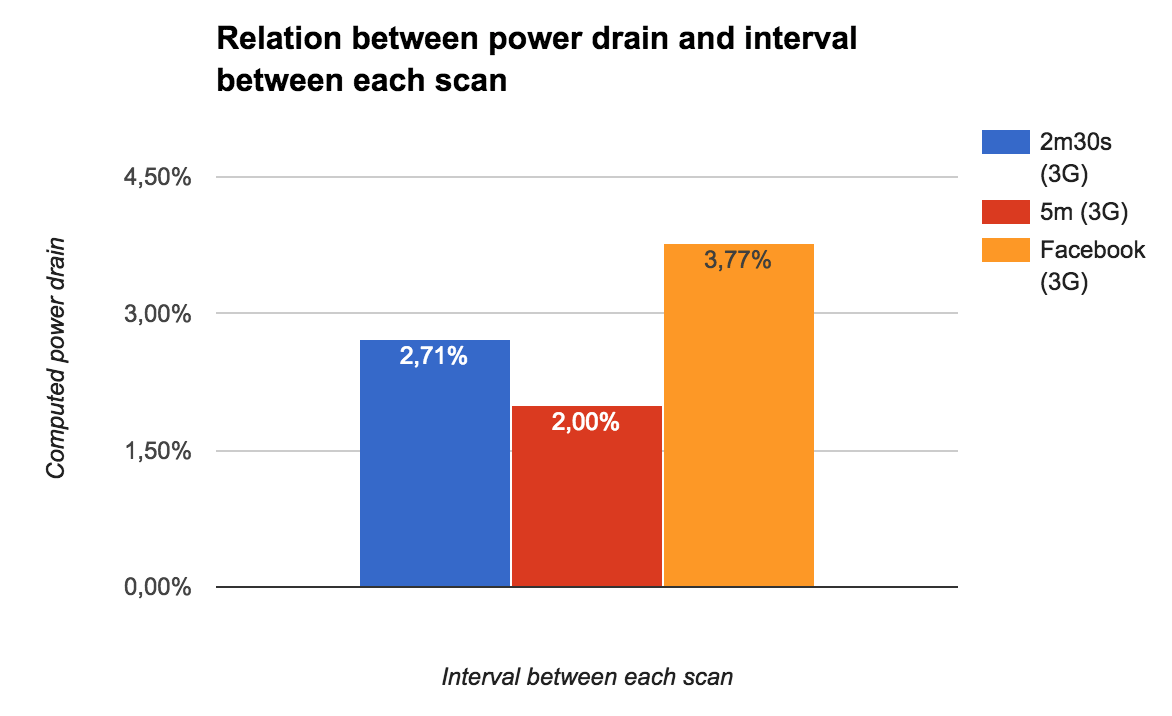
\includegraphics[width=0.8\textwidth, keepaspectratio]{images/results_battery_walking}
    \caption[Power drain when the user is moving]{Relation between power drain and interval between each scan in the scenario where the user moves along multiple Smart Places}
    \label{fig:results_battery_walking}
\end{figure}

Looking at the results, it is possible to establish a relation between power drain and data transferred (sent and received).
In all experiments, we measured how many \gls{KB} were transferred.
Since, when using \gls{WiFi}, the power drain was almost zero, we have focused in the relation between power drain and data transferred using \gls{3G}.
As the graphic, in Figure~\ref{fig:results_battery_data}, shows, as more data is transferred, more power, of the mobile device, is drained.
It is possible to conclude that, the more our mobile app needs to communicate with the backend, the more is the energy consumption.

\begin{figure}[!ht]
  \centering
    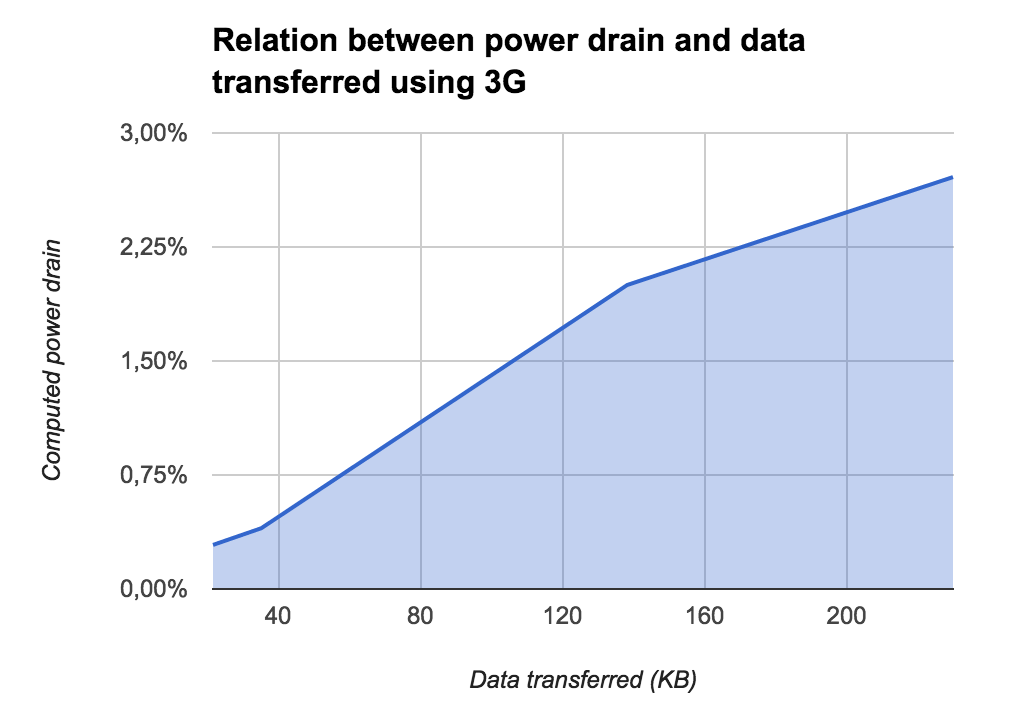
\includegraphics[width=0.8\textwidth, keepaspectratio]{images/results_battery_data}
    \caption[Power drain vs Data transferred]{Relation between power drain and data transferred}
    \label{fig:results_battery_data}
\end{figure}

\section{Summary}
\label{sec:evaluation_summary}
% Setup
% -> Smartphone and 3 beacons of Estimote
% Two kinds of experiments
After developing the Smart Places solution, we performed an evaluation.
We have used a \tm{Motorola} Moto G smartphone and three beacons from \tm{Estimote} and we performed two sets of experiments.

% Nearest beacon
% -> What and why
% -> Comment results
The mobile app for end users scans for nearby beacons and requests information, to the backend, about the one that is less distant to the mobile device.
Somehow, the app needs to be able to get the distance from a given beacon.
Our mobile apps project used a library to handle the \gls{BLE} beacons. This library has a method to get the distance, from a given beacon, that was previously scanned.
However, we performed experiments in order to see if it is possible to trust this value.
Our experiments showed that, to build applications that rely on detecting the nearest beacon, the beacons need to be, at least, 1.5m distant from each other.
As we raise the distance between beacons, the nearest beacon is successfully detected.

% Energy consumption
% -> What and why
% -> Comment results
The mobile app for end users scans for nearby beacons in background.
As any service running in background, it can introduce an overhead in terms of energy consumption.
We performed a set of experiments to get the power drain and data transferred (sent and received) by the mobile app.
To get the power drain and data transferred values we used Battery Historian tool.
We have tested two different scenarios. A scenario where the user stays in the same Smart Place and another one where he is always moving from one Smart Place to another.
Each experiment runned for one hour.
For each scenario, we tested \gls{WiFi} and \gls{3G} as data connection means.
The results showed that the power drain is bigger when using \gls{3G}. When using \gls{WiFi}, the power drain is almost zero.
In the scenario where the user does not move, the power drain is less than 1\%.
However, in the scenario where the user is always moving, which implies more requests to the backend, because new Smart Places are detected in each new scan, the power drain can be more than 2\%.
This can compromise the usability of our solution because, assuming a linear growth of power drain, in 24 hours, our mobile app would drain 48\%.
Having into account that most users already have apps that require a data connection, this can be unnaceptable in most cases.
In the end, we related data transferred with power drain and the results showed that unsurprisingly as more data is transferred (sent and received), more power is drained.
